\sectionwithlogo{Компьютерная графика}
{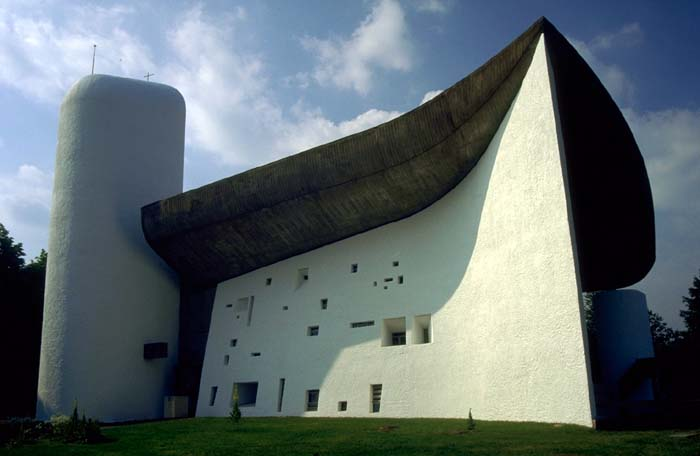
\includegraphics[width=.75\textwidth]{figure-ronchamp}\\
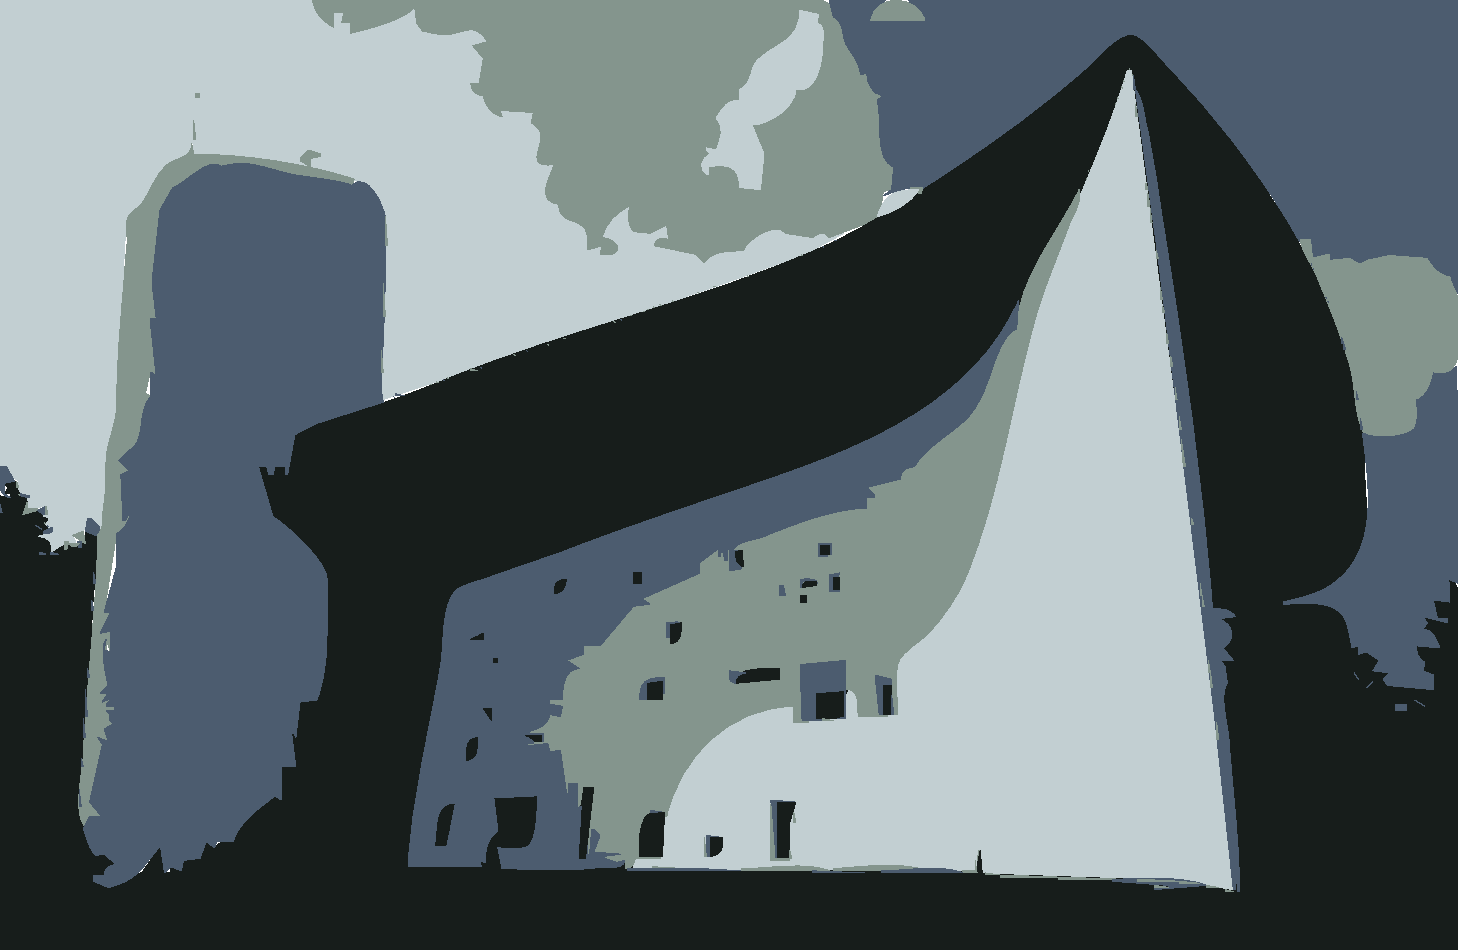
\includegraphics[width=.75\textwidth]{figure-ronchamp-4}}

%%%%%%%%%%

\begin{frame}{Растровая графика}
\centerline{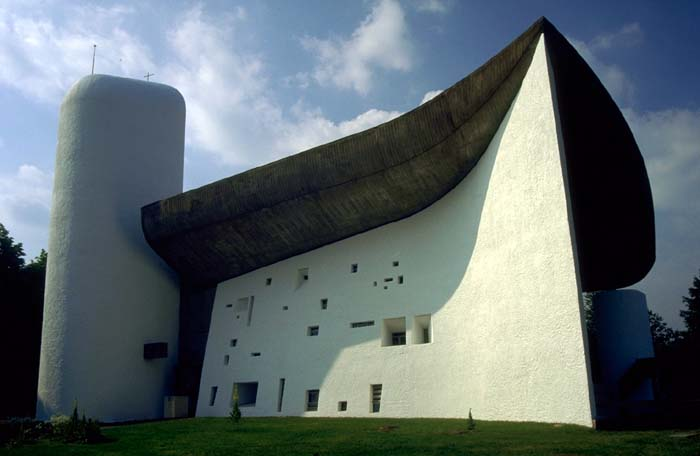
\includegraphics[scale=.2]{figure-ronchamp}}
\begin{itemize}
\item изображение формируется как прямоугольный массив точек (пикселов)
\item наиболее подходит для фотоизображений
\item популярные форматы: PNG, JPEG, GIF, PCX, BMP,~…
\item популярные программы обработки изображений: Adobe~PhotoShop, The Gimp,~…
\item плохо переносит масштабирование и~вращение
\end{itemize}
\end{frame}

%%%%%%%%%%

\begin{frame}{Векторная графика}
\label{vector}
\begin{columns}
\column{.33333\textwidth}

\includegraphics[scale=.0625]{aiga_litter_disposal1}

\includegraphics[scale=.0625]{aiga_fire_extinguisher1}

\includegraphics[scale=.0625]{aiga_immigration1}\\

\includegraphics[scale=.0625]{aiga_hotel_information1}

\includegraphics[scale=.0625]{aiga_heliport1}

\includegraphics[scale=.0625]{aiga_ground_transportation1}\\

\includegraphics[scale=.0625]{aiga_rail_transportation1}

\includegraphics[scale=.0625]{aiga_drinking_fountain1}

\includegraphics[scale=.0625]{aiga_lost_and_found1}\\

\includegraphics[scale=.0625]{aiga_nursery1}

\includegraphics[scale=.0625]{aiga_restaurant1}

\includegraphics[scale=.0625]{aiga_toilets1}\\

\includegraphics[scale=.0625]{aiga_waiting_room1}

\includegraphics[scale=.0625]{aiga_tickey_purchase1}

\includegraphics[scale=.0625]{aiga_smoking1}\\

\includegraphics[scale=.0625]{aiga_shops1}

\includegraphics[scale=.0625]{aiga_bus1}

\includegraphics[scale=.0625]{aiga_departing_flights1}\\

\includegraphics[scale=.0625]{aiga_customs1}

\includegraphics[scale=.0625]{aiga_barber_shop1}

\includegraphics[scale=.0625]{aiga_baggage_check_in1}
\column{.75\textwidth}
\begin{itemize}
\item изображение формируется из графических примитивов (линий, фигур, надписей)
\item наиболее подходит для чертежей, графиков, диаграмм
\item популярные форматы: SVG, PostScript, PDF,~…
\item популярные программы обработки изображений: CorelDraw, InkScape,~…
\item отлично переносит масштабирование и~вращение
\end{itemize}
\end{columns}
\end{frame}

%%%%%%%%%%

\begin{frame}{Трассировка и~растеризация}
\begin{center}
\Huge
$\text{растр}
{\xrightarrow{\text{трассировка}}\atop\xleftarrow[\text{растеризация}]{}}
\text{вектор}$
\end{center}
\end{frame}

%%%%%%%%%%

\begin{frame}{Растеризация}
\begin{columns}
\column{.5\textwidth}
\includeMPgraphics{figure-rasterize-1}\\[4ex]
\includeMPgraphics{figure-rasterize-3}
\column{.5\textwidth}
\includeMPgraphics{figure-rasterize-2}\\[4ex]
\includeMPgraphics{figure-rasterize-4}
\end{columns}
\end{frame}

%%%%%%%%%%

\begin{frame}{Растеризация}
Результат зависит:
\begin{itemize}
\item от разрешения (размера клеток решётки)
\item от положения фигуры на решётке
\item от того, считать точки на границе фигуры её частью, или нет
\end{itemize}

Чем выше разрешение, тем лучше результат.
\end{frame}

%%%%%%%%%%

\begin{frame}{Сглаживание (antialiasing)}
\begin{columns}
\column{.5\textwidth}
\includeMPgraphics{figure-antialiasing-1}\\[4ex]
\includeMPgraphics{figure-antialiasing-2}
\column{.5\textwidth}
\begin{itemize}
\item
измельчается решётка в~2~раза (иногда в~4 или 8~раз)
\item
для каждой крупной клетки подсчитывается доля мелких клеток, задевающих фигуру
\item
крупная клетка закрашивается цветом пропорционально найденной доле
\end{itemize}
\end{columns}
\end{frame}

%%%%%%%%%%

\begin{frame}{Сглаживание (antialiasing)}
Сглаживание изображений букв в~программах компьютерной вёрстки устроено
сложнее.

В~частности, особого подхода требуют прямолинейные горизонтальные или
вертикальные участки границы буквы.

Для лучшего качества на таких участках сглаживание подавляется.
\end{frame}

%%%%%%%%%%

\begin{frame}{Трассировка (векторизация)}
\begin{columns}
\column{.6\textwidth}
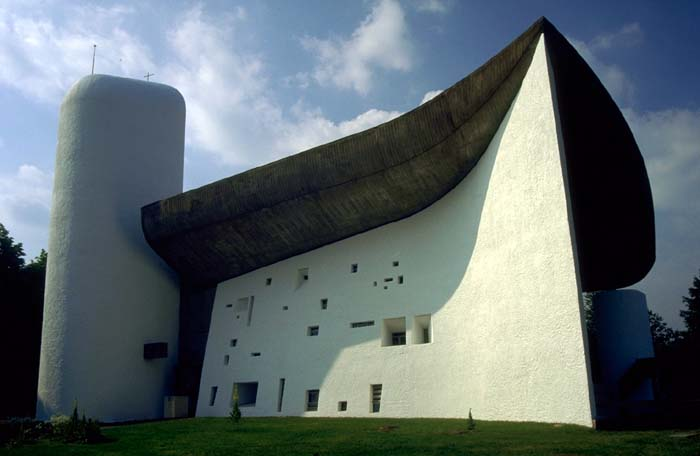
\includegraphics[scale=.24]{figure-ronchamp}
\column{.4\textwidth}

\includegraphics[scale=.1]{figure-ronchamp-2}\enspace{\scriptsize 2 цвета}\\[1ex]
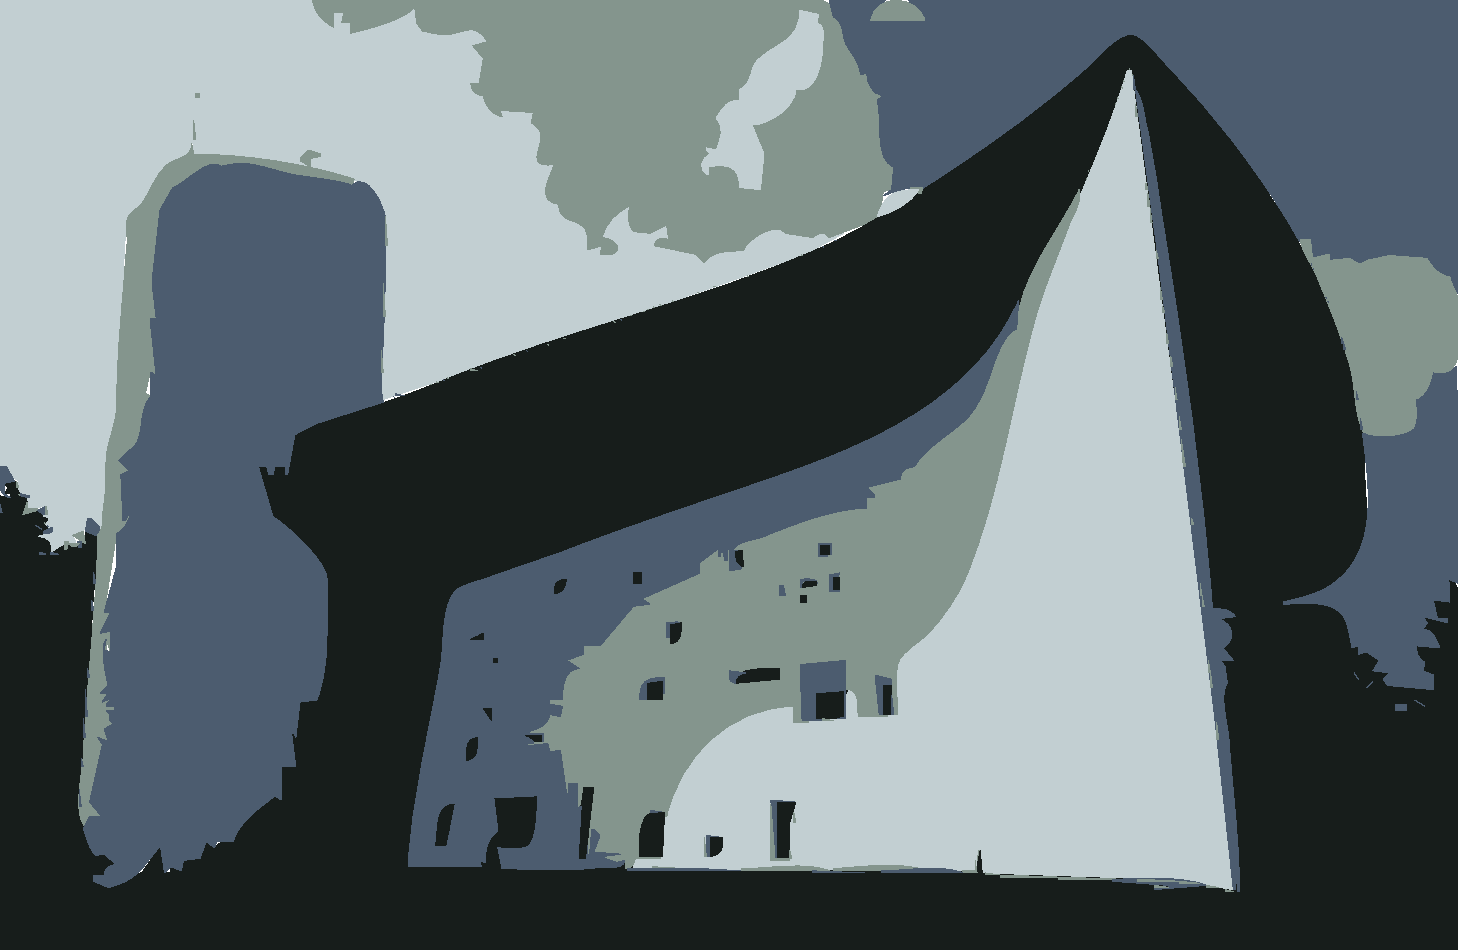
\includegraphics[scale=.1]{figure-ronchamp-4}\enspace{\scriptsize 4 цвета}\\[1ex]
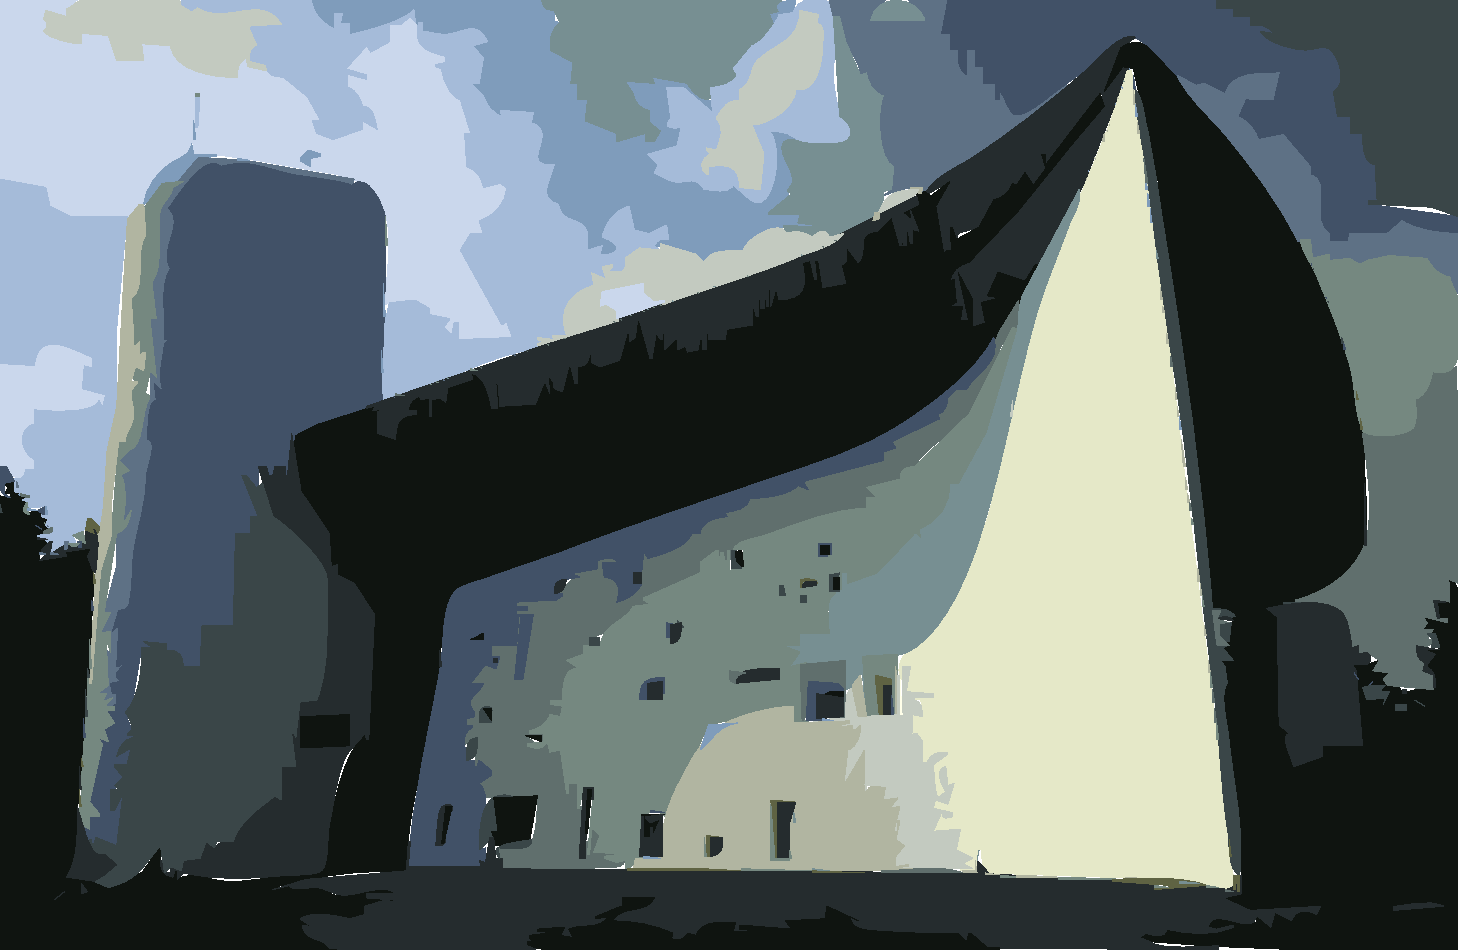
\includegraphics[scale=.1]{figure-ronchamp-16}\enspace{\scriptsize 16 цветов}\\[1ex]
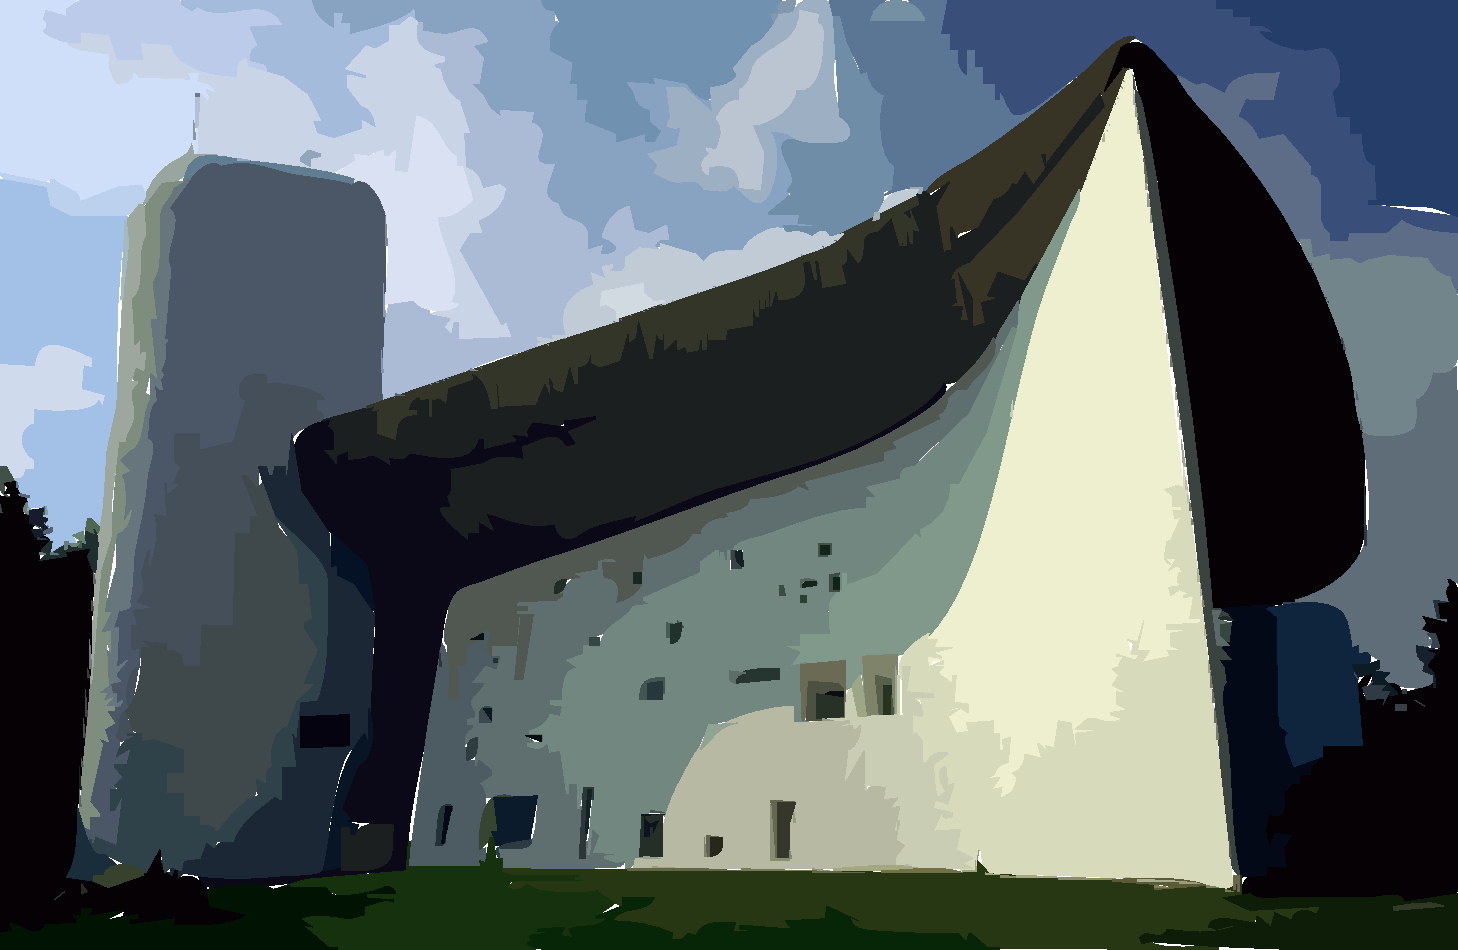
\includegraphics[scale=.1]{figure-ronchamp-256}\enspace{\scriptsize 256 цветов}
\end{columns}
\end{frame}
